\documentclass[9pt,t,aspectratio=169]{beamer}
\usetheme[white]{Wisconsin}
\usepackage[utf8]{inputenc}
\setbeamertemplate{page number in head/foot}[totalframenumber]
\setbeamerfont{title}{size=\LARGE}
\setbeamerfont{subtitle}{size=\Large}
\setbeamerfont{block body}{size=\footnotesize}
\setbeamerfont{author}{size=\LARGE}
\setbeamerfont{date}{size=\Large}
\setbeamerfont{institute}{size=\large}
\setlength{\leftmargini}{0pt}


\usepackage{caption}
\captionsetup[figure]{labelformat=empty} % turn off labeling caption figures
%subcaptions
\usepackage{subcaption}
\captionsetup[subfigure]{labelformat=empty} % turn off labeling subcaption figures

% turn off Figure in captions
\usepackage{caption}
% \captionsetup[figure]{labelformat=empty}

\newcommand{\QOR}{\qquad \text{OR} \qquad}
\newcommand{\QAND}{\qquad \text{AND} \qquad}
\newcommand{\QTHUS}{\qquad \text{THUS} \qquad}
\newcommand{\QTHEN}{\qquad \text{THEN} \qquad}
\newcommand{\QWITH}{\qquad \text{WITH} \qquad}
\newcommand{\QFOR}{\qquad \text{FOR} \qquad}
\newcommand{\QSO}{\qquad \text{SO} \qquad}
\newcommand{\QWHERE}{\qquad \text{WHERE} \qquad}
\newcommand{\LINE}{\par\noindent\rule{\textwidth}{0.4pt}\par}
\newcommand{\toinf}{\rightarrow\infty}
\newcommand{\tozero}{\rightarrow0}
\newcommand{\qeq}{\overset{?}{=}}
\newcommand{\ceq}{\overset{\checkmark}{=}}
\renewcommand{\epsilon}{\varepsilon}
\newcommand{\keff}{$k_{e\!f\!f}$}
\newcommand{\kinf}{$k_{inf}$}

% table packages
\usepackage{booktabs}

% Roman Numerals
\newcommand{\rom}[1]{\expandafter\uppercase{\Romannumeral #1\relax}}

% hypersetup
\usepackage{hyperref}
\hypersetup{colorlinks,
            linkcolor = black,
            citecolor = black,
            urlcolor = cyan
}


\def\brac#1{\{#1\}}
\def\Brac#1{\big\{#1\big\}}
\def\BRAC#1{\bigg\{#1\bigg\}}
\def\angbrac#1{\langle#1\rangle}
\def\Angbrac#1{\big\langle#1\big\rangle}
\def\ANGBRAC#1{\bigg\langle#1\bigg\rangle}

% Transitional slides between sections
\AtBeginSection[]
{
    \begin{frame}
        \frametitle{Table of Contents}
        \tableofcontents[currentsection]
    \end{frame}
}


% Bibliography
\usepackage[sorting=none]{biblatex} %Imports biblatex package and cites in order of appearance
\addbibresource{physor2024_pres.bib} %Import the bibliography file
% make all font colors white
\setbeamercolor{bibliography item}{fg=black}
\setbeamercolor{bibliography entry author}{fg=black}
\setbeamercolor{bibliography entry title}{fg=black}
\setbeamercolor{bibliography entry location}{fg=black}
\setbeamercolor{bibliography entry note}{fg=black}
% adds numeric labels linked to bib entries
\setbeamertemplate{bibliography item}{\insertbiblabel}

% eliminate header within an environment
\makeatletter
    \newenvironment{withoutheadline}{
       \setbeamertemplate{headline}[default]
       \def\beamer@entrycode{\vspace*{-\headheight}}
    }{}
\makeatother

% appendix renumbering
\usepackage{appendixnumberbeamer}
% frame breaks with same title
\setbeamertemplate{frametitle continuation}[from second][]

\title{Exploring Effects of Homogenization on an OpenMC Depletion Analysis}
\subtitle{of a TRISO Fueled, Helium Cooled Microreactor}
\author{\vspace*{-0.45cm}Lewis I. Gross\textsuperscript{1}, Patrick Shriwise\textsuperscript{2,1}, Benjamin Lindley\textsuperscript{1} and Paul P.H. Wilson\textsuperscript{1}}
\institute{University of Wisconsin-Madison\textsuperscript{1}, Argonne National Lab\textsuperscript{2} }
\date{\vspace*{-0.25cm}April 24, 2024}
%%----------------------------------------------------------------------------%%
\begin{document}

\begin{withoutheadline}
\begin{frame}[plain] % the plain makes the first frame look good
    \maketitle
\end{frame}
\end{withoutheadline}

\author{Lewis Gross, Patrick Shriwise, Ben Lindley, and Paul Wilson} % reset author so affiliations don't show up in footer
%%----------------------------------------------------------------------------%%
%% Overview
%%----------------------------------------------------------------------------%%
\begin{withoutheadline}
\begin{frame}{Outline}
  \tableofcontents
\end{frame}
\end{withoutheadline}


%%----------------------------------------------------------------------------%%
%% Section 1
%%----------------------------------------------------------------------------%%
\section{Virtual Test Bed Gas-Cooled Microreactor}
\hypersetup{citecolor=white}
\begin{withoutheadline}
\begin{frame}{Virtual Test Bed \cite{vtb2023}}
    \begin{figure}
        \centering
        
\includegraphics[width=0.5\linewidth]{figures/nric_logo.png}
    \end{figure}
    \begin{figure}
        \centering
        
\includegraphics[width=0.5\linewidth]{figures/NEAMS.png}
    \end{figure}
    \begin{figure}
        \centering
        
\includegraphics[width=0.5\linewidth]{figures/moose_logo.png}
    \end{figure}
\end{frame}
\end{withoutheadline}

\begin{withoutheadline}
\begin{frame}{Microreactors \cite{INL_MR}}
    \begin{figure}
        \pause
        \centering
        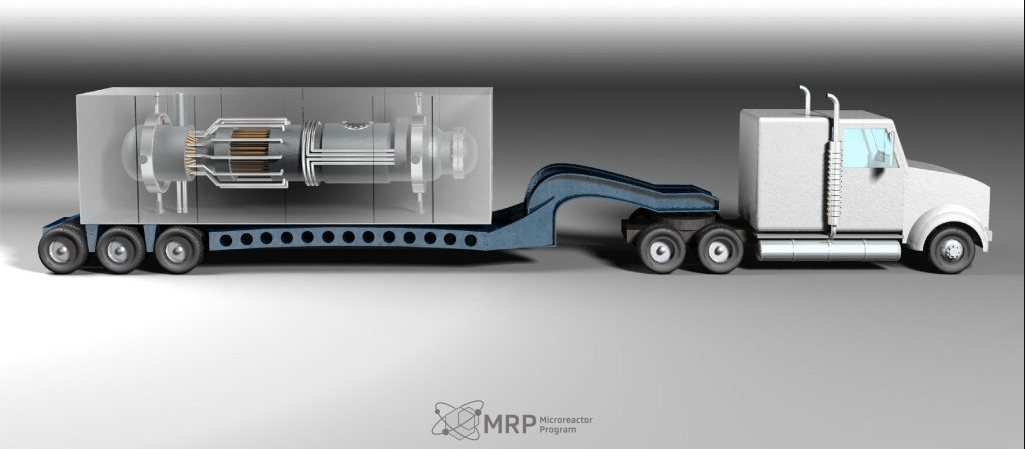
\includegraphics[width=0.8\linewidth]{figures/INL_MR.png}
    \end{figure}
\end{frame}
\end{withoutheadline}
\hypersetup{citecolor=black}

\begin{withoutheadline}
\begin{frame}{High Temperature Gas Reactors and TRISO Fuel}
    \begin{minipage}[t]{0.4\linewidth}
        \pause
        \begin{figure}
            \centering
            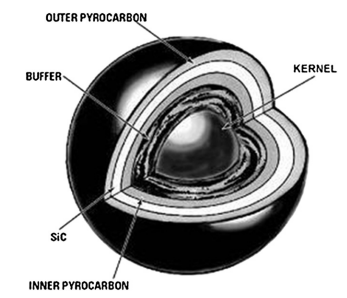
\includegraphics[width=0.9\linewidth]{figures/TRISO_diagram_Zhou_Tang.png}
            \caption{Image from \cite{zhou_tang}}
        \end{figure}
    \end{minipage}
    \hfill%
    \begin{minipage}[t]{0.575\linewidth}
        \pause
        \LARGE
        \begin{itemize}
            \item <3-> TRISO fuel synergizes with HTGRs
            \begin{itemize}
                \Large
                \item <3-> Melting temperature significantly higher than operational temperatures \cite{zhou_tang}
                \item <3-> Designed to contain fission products \cite{zhou_tang}
                \item <3-> Typically packed into graphite compacts or into spherical pebbles for PBRs
            \end{itemize}
            \item <4-> TRISO modeling challenges
            \begin{itemize}
                \Large
                \item <4-> Five surfaces per TRISO
                \item <4-> Causes very many surface crossings per history
                \item <4-> High memory requirement for fully explicit representation
            \end{itemize}
        \end{itemize}
        \normalsize
    \end{minipage}
\end{frame}
\end{withoutheadline}

\begin{withoutheadline}
\begin{frame}{Virtual Test Bed Gas Cooled Microreactor (VTB GCMR)}
    \pause
    \LARGE
    \begin{minipage}[t]{0.55\linewidth}
        \begin{itemize}
            \item<2-> Existing simulations using MOOSE tools
            \begin{itemize}
                \Large
                \item<2-> Griffin-BISON-SAM multiphysics models, including accident and load-following transients:  \cite{Stauff-applications-2022,Abdelhameed-ANS-2022, HF_MRs_ANL}
                \item<2-> Balance of plant 1D thermal hydraulic simulation \cite{Duchnowski_plant_balance_2022}
            \end{itemize}
            \item<3-> This work presents the first published OpenMC Model of the VTB GCMR
            \begin{itemize}
                \Large
                \item<3->Plans to add this work's model to the VTB this summer
            \end{itemize}
            \item<4-> For a full core model, it will be prohibitively expensive to model every TRISO explicitly
            \begin{itemize}
                \Large
                \item<4-> $O(10^{13})$ per assembly
            \end{itemize}
        \end{itemize}
    \end{minipage}
    \hfill%
    \begin{minipage}[t]{0.4\linewidth}
        \begin{figure}
            \centering
            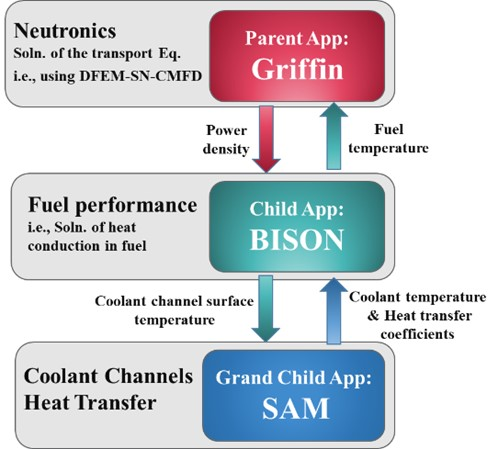
\includegraphics[width=\linewidth]{figures/gcmr_preliminary_mutliapps.png}
            \caption{MultiApp hierarchy of preliminary GCMR models. Image from \cite{Abdelhameed-ANS-2022}.}
        \end{figure}
    \normalsize
    \end{minipage}
\end{frame}
\end{withoutheadline}

\begin{withoutheadline}
\begin{frame}{Research Question}
    \pause
    \begin{itemize}
        \item<2-> \textbf{In order to balance performance and fidelity, what degree of TRISO homogenization is allowable to accurately compute the k-eigenvalue as a function of burnup for whole core Monte Carlo modeling?}
        \item<3-> Two homogenization strategies:``\textbf{kernel only}'' and ``\textbf{full volume}''
        \begin{figure}
            \pause
            \begin{subfigure}{0.3\linewidth}
                \centering
                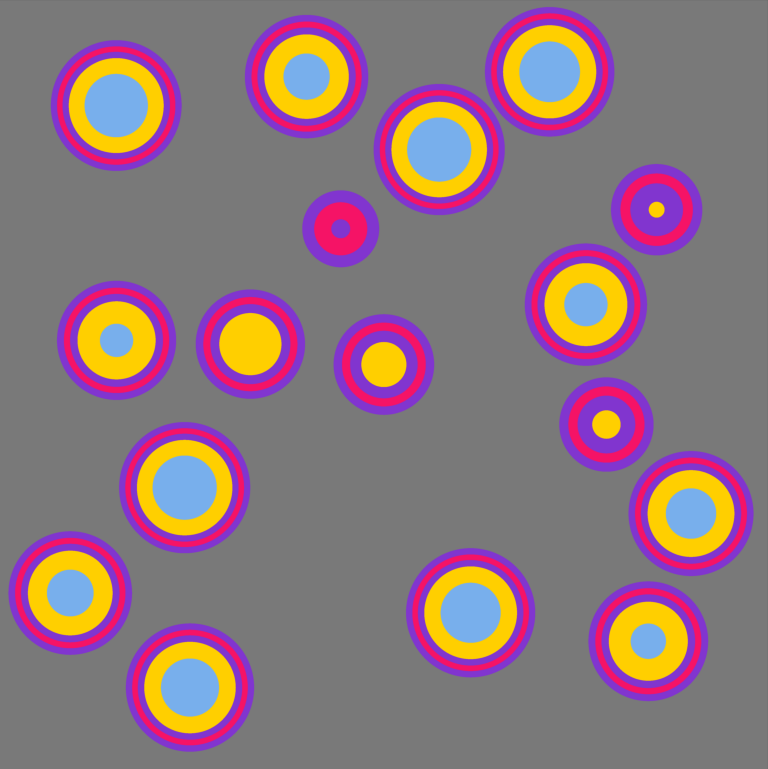
\includegraphics[width=\linewidth]{figures/explicit_viz.png}
                \caption{explicit}
            \end{subfigure}
            \begin{subfigure}{0.3\linewidth}
                \centering
                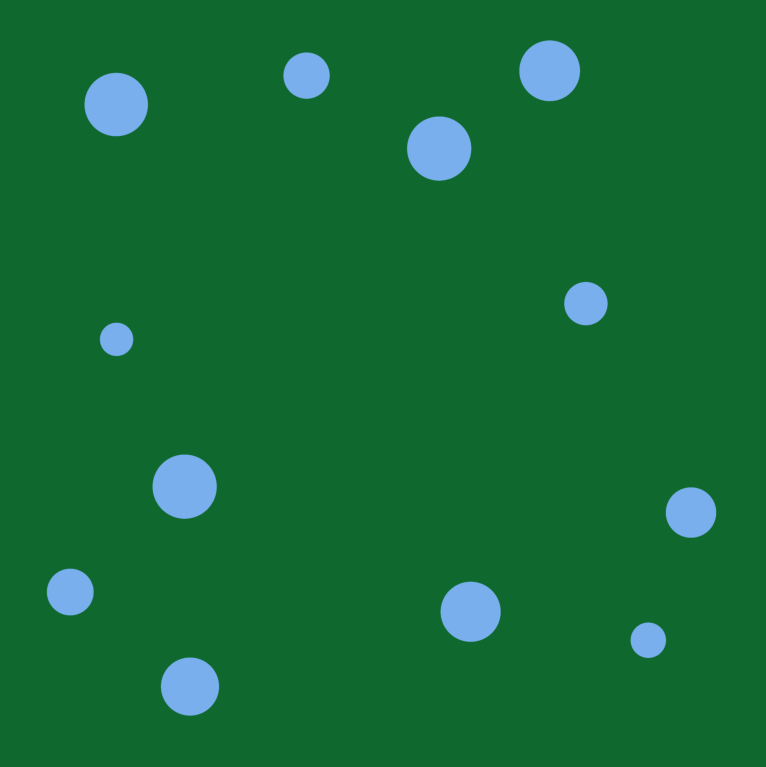
\includegraphics[width=\linewidth]{figures/kern_viz.png}
                \caption{kernel only}
            \end{subfigure}
            \begin{subfigure}{0.3\linewidth}
                \centering
                
\includegraphics[width=\linewidth]{figures/homog_viz.png}
                \caption{full volume}
            \end{subfigure}
        \end{figure}
        \item<4-> Burnup simulations at 100\%, 50\%, and 10\% of full power (225 KWt)
        \item<4-> Compare each \kinf~as a basis for deciding how proceed with a full core model
    \end{itemize}
\end{frame}
\end{withoutheadline}

%%----------------------------------------------------------------------------%%
%% Section 2
%%----------------------------------------------------------------------------%%
\section{OpenMC Model}
\begin{withoutheadline}
\hypersetup{citecolor=white}
\begin{frame}{OpenMC Infinite Assembly Model: Images via openmc-plotter \cite{openmc-plotter}}
    \begin{minipage}[t]{0.225\linewidth}
        \pause
        \begin{figure}
            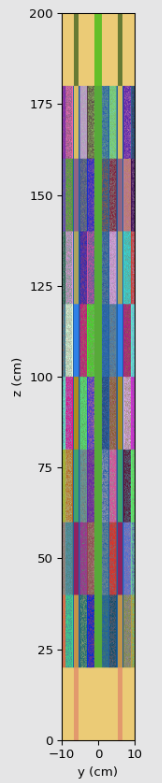
\includegraphics[height=0.8\textheight]{figures/yz_slice.png}
            \caption{YZ slice of reactor}
        \end{figure}
    \end{minipage}
    \begin{minipage}[t]{0.45\linewidth}
        \pause
        \begin{figure}
            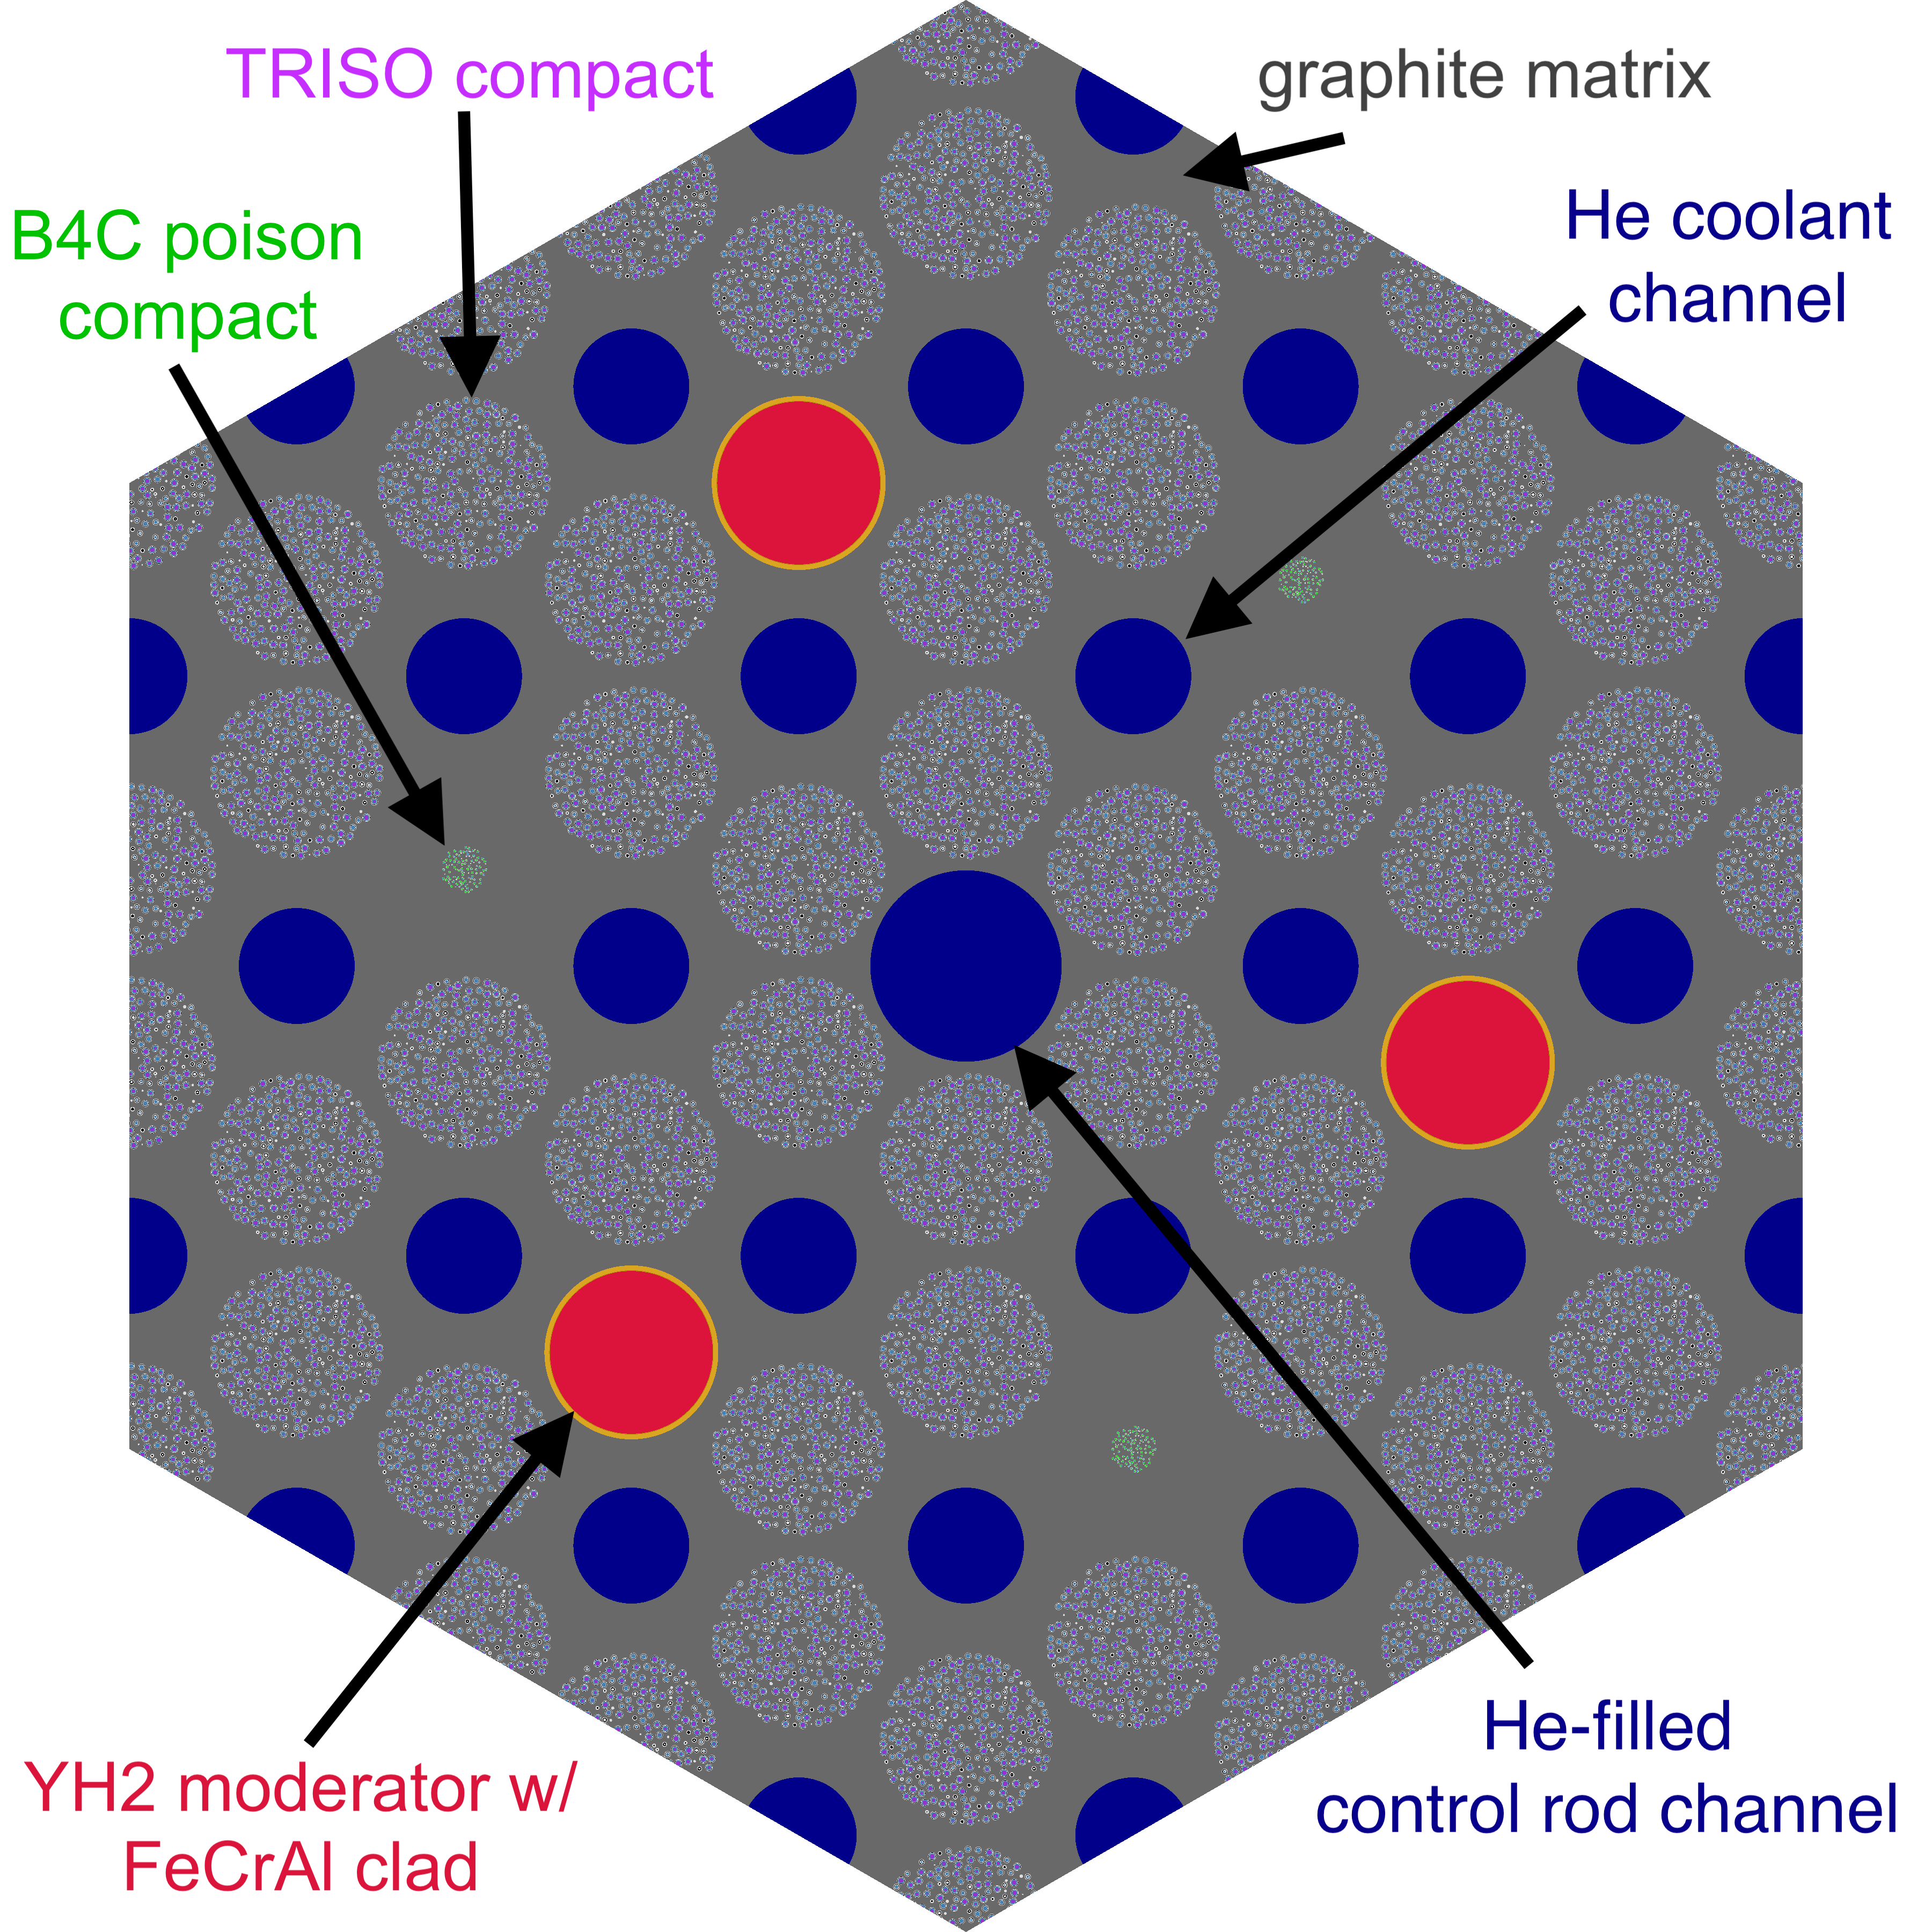
\includegraphics[height=0.8\textheight]{figures/gcmr_labeled_slice.png}
            \caption{XY slice of reactor}
        \end{figure}
    \end{minipage}
    \hfill%
    \begin{minipage}[t]{0.3\linewidth}
        \Large
        \begin{itemize}
            \item<4-> spatial depletion scheme
            \item<4-> 3-way radial symmetry cloning scheme
            \item<4-> 8 axial layers in the core
            \item<4-> 2 axial layers per reflector
        \end{itemize}
        \normalsize
    \end{minipage}
\end{frame}
\hypersetup{citecolor=black}
\end{withoutheadline}

\begin{withoutheadline}
\begin{frame}{OpenMC Depletion Settings}
    \pause
    \LARGE
    \begin{itemize}
        \item<2-> Constant Extrapolation/Constant Midpoint (CE/CM) time integration scheme from Isotalo et al. \cite{isotalo_comparison_2015}
        \begin{itemize}
            \Large
            \item<2-> 25 inactive and 75 active batches with 10000 particles per batch
            \item<2-> continuous energy cross sections from ENDF-B-VII.1
        \end{itemize}
        \item<3-> CASL project \cite{CASL-report} chain XML file, provided by OpenMC \cite{openmc-chains}
        \begin{itemize}
            \Large
            \item<3-> Contains transmutation and decay data necessary to compute the burnup matrix
        \end{itemize}
        \item<4-> Time Steps
        \begin{itemize}
            \Large
            \item<4-> Full power time steps: \texttt{[1]*5 + [5]*3 + [15]*3 + [60]*17} (days)
            \item<4-> Burnup-consistent time steps for other powers
        \end{itemize}
    \end{itemize}
    \normalsize
\end{frame}
\end{withoutheadline}
%%----------------------------------------------------------------------------%%
%% Section 3
%%----------------------------------------------------------------------------%%
\section{Results and Discussion}

\begin{withoutheadline}
\begin{frame}{Fully-explicit \kinf~versus burnup with $2\sigma$ error bars up to $\sim$29 GWd/tonne-U}
    \begin{figure}
        \vspace*{-0.4cm}
        \centering
            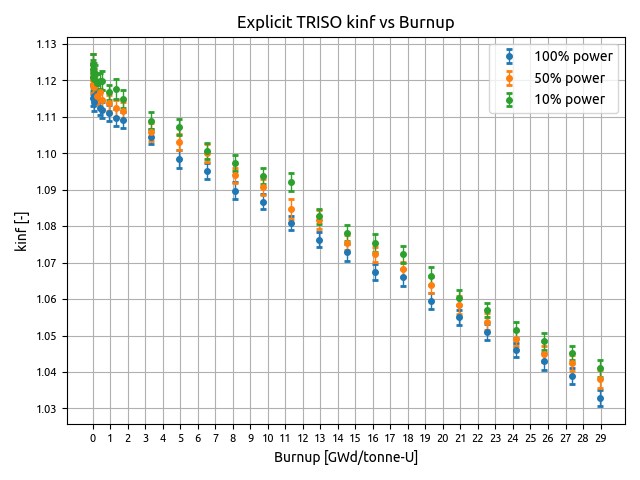
\includegraphics[height=\textheight]{figures/expl_kinf_vs_bu.png}
        \label{fig:kinf_full_explicit_results}
    \end{figure}
\end{frame}
\end{withoutheadline}

\begin{withoutheadline}
\begin{frame}{Comparing Eigenvalues}
    \pause
    \Large
    \begin{itemize}
        \item<2-> Denote the first set of eigenvalues $k_ 1$ and the second set $k_2$, the $\Delta \rho$ between them is given by
        \begin{equation}
            \Delta \rho \equiv
            \rho_1 - \rho_2 =
            \frac{k_1-1}{k_1} - \frac{k_2 - 1 }{k_2} =
            \frac{1}{k_2} - \frac{1}{k_1}
        \end{equation}
        \item<3-> Average $\Delta \rho$ compared with the explicit reference at every power with $2\sigma$ uncertainties
        \begin{table}[!h]
            \centering
            \begin{tabular}{c|c|c}
            $\overline{\Delta \rho}$ & explicit - homogenized & explicit - kernel only \\ \hline
            100\% power & 1533 $\pm$ 55 pcm &  -158 $\pm$ 55 pcm \\
            50\% power & 1495 $\pm$ 56 pcm & -193 $\pm$ 55 pcm\\
            10\% power & 1529 $\pm$ 56 pcm  & -203 $\pm$ 55 pcm
            \end{tabular}
            \label{tab:average_pcms}
        \end{table}
    \item<4-> Kernel only $\Delta \rho$ on average performs about 1 order of magnitude better than full homogenization.
    \end{itemize}
    \normalsize
\end{frame}
\end{withoutheadline}

%%----------------------------------------------------------------------------%%
%% Section 4
%%----------------------------------------------------------------------------%%
\section{Next Steps}
\begin{withoutheadline}
\begin{frame}{Two-layer TRISO Homogenization}
    \pause
    \begin{itemize}
        \item<2-> While the kernel only eigenvalue computation outperforms the fully homogenized in terms of accuracy, it would be desirable to lower $\Delta \rho$ below 100 pcm.
        \item<3-> The kernel only model moves SiC further from the fuel than it exists in the explicit model.
        \item<3-> Si is less efficient at thermalizing neutrons and absorbs more neutrons than C.
        \item<4-> A next iteration on fuel homogenization would be to create a \textbf{two layer} homogenization
    \end{itemize}
    \begin{figure}
        \pause
        \pause
        \begin{subfigure}{0.3\linewidth}
            \centering
            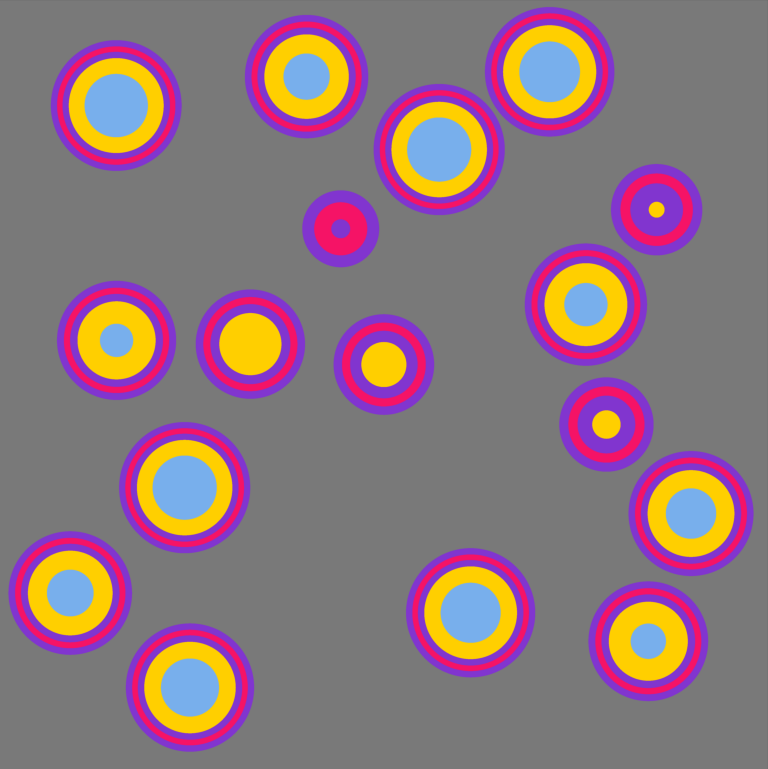
\includegraphics[width=\linewidth]{figures/explicit_viz.png}
            \caption{explicit}
        \end{subfigure}
        \begin{subfigure}{0.3\linewidth}
            \centering
            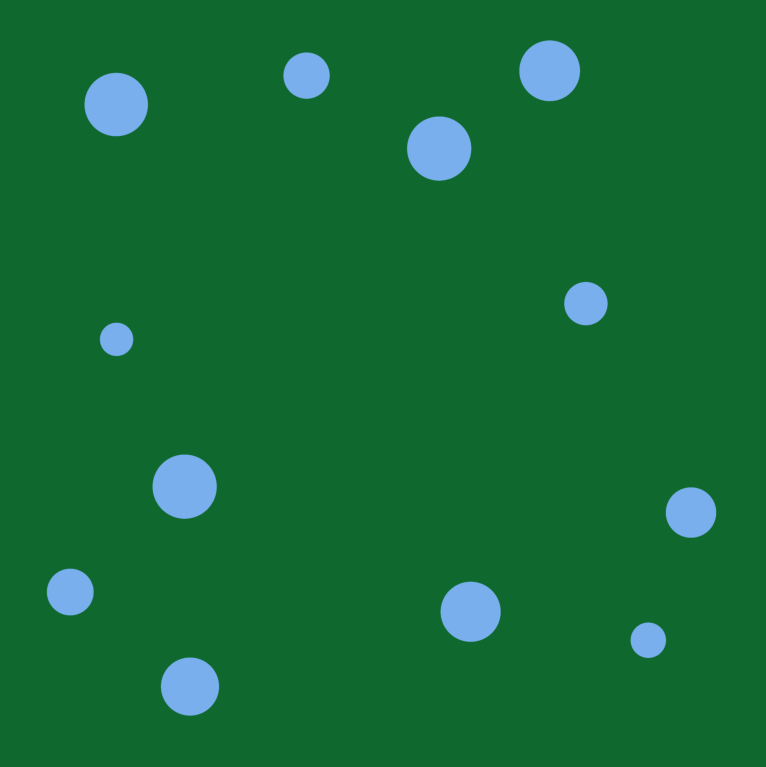
\includegraphics[width=\linewidth]{figures/kern_viz.png}
            \caption{kernel only}
        \end{subfigure}
        \begin{subfigure}{0.3\linewidth}
            \centering
            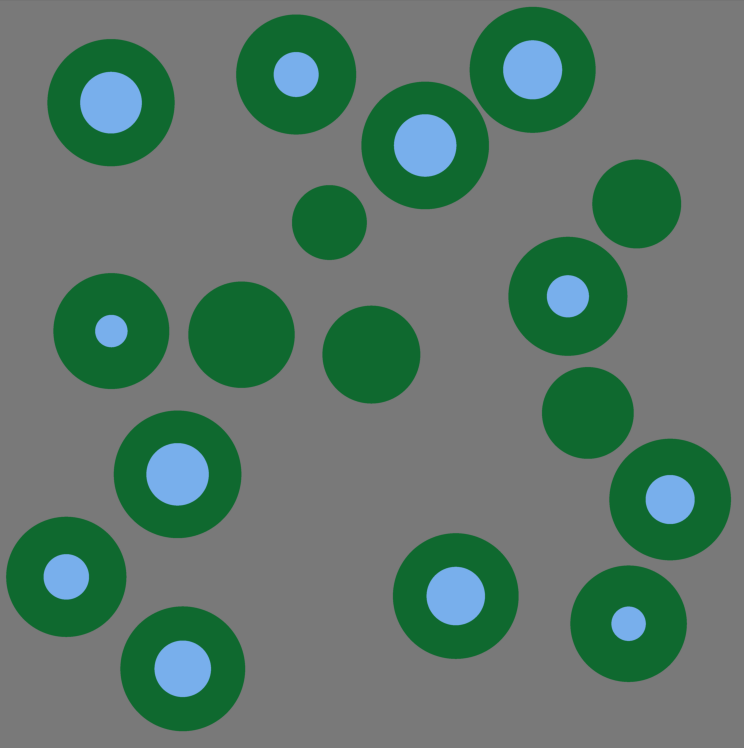
\includegraphics[width=\linewidth]{figures/2layer_viz.png}
            \caption{two layer TRISO}
        \end{subfigure}
    \end{figure}
\end{frame}
\end{withoutheadline}

%%----------------------------------------------------------------------------%%`'
%% Bibliography
%%----------------------------------------------------------------------------%%

\begin{withoutheadline}
    \begin{frame}{Acknowledgements}
        \begin{itemize}
            \item The first author was supported in part by the US Nuclear Regulatory Commission's Graduate Fellowship Program administered by the University of Wisconsin-Madison.
            \item The OpenMC team!
            \item The Center for High Throughput Computing at the University of Wisconsin - Madison
            \item Co-authors: Patrick Shriwise, Benjamin Lindley, and Paul P.H.~Wilson.
        \end{itemize}
        \begin{figure}[H]
            \centering
            
\includegraphics[height=0.3\textheight]{figures/openmc_logo.png}
        \end{figure}
        \begin{figure}[H]
            \centering
            
\includegraphics[height=0.3\textheight]{figures/CHTC.png}
        \end{figure}
    \end{frame}
\end{withoutheadline}

\begin{withoutheadline}
    \begin{frame}[allowframebreaks]{Bibliography}
        \printbibliography
    \end{frame}
\end{withoutheadline}

\begin{withoutheadline}
    \begin{frame}{Open Source Projects}
        \begin{minipage}[t]{0.43\linewidth}
            \begin{itemize}
                \item OpenMC website: \href{https://openmc.org}{https://openmc.org}
                \item OpenMC repository: \href{https://github.com/openmc-dev/openmc}{https://github.com/openmc-dev/openmc}
                \item OpenMC plotter: \href{https://github.com/openmc-dev/plotter}{https://github.com/openmc-dev/plotter}
                \item VTB: \href{https://mooseframework.inl.gov/virtual_test_bed}{https://mooseframework.inl.gov/virtual\_test\_bed}
                \item VTB repository: \href{https://github.com/idaholab/virtual_test_bed}{https://github.com/idaholab/virtual\_test\_bed}
                \item Add me on LinkedIn (\href{https://www.linkedin.com/in/lewisgross1296}{lewisgross1296}) and GitHub (\href{https://github.com/lewisgross1296}{lewisgross1296})!
            \end{itemize}
        \end{minipage}
        \hfill% 
        \begin{minipage}[t]{0.54\linewidth}
            \begin{figure}
                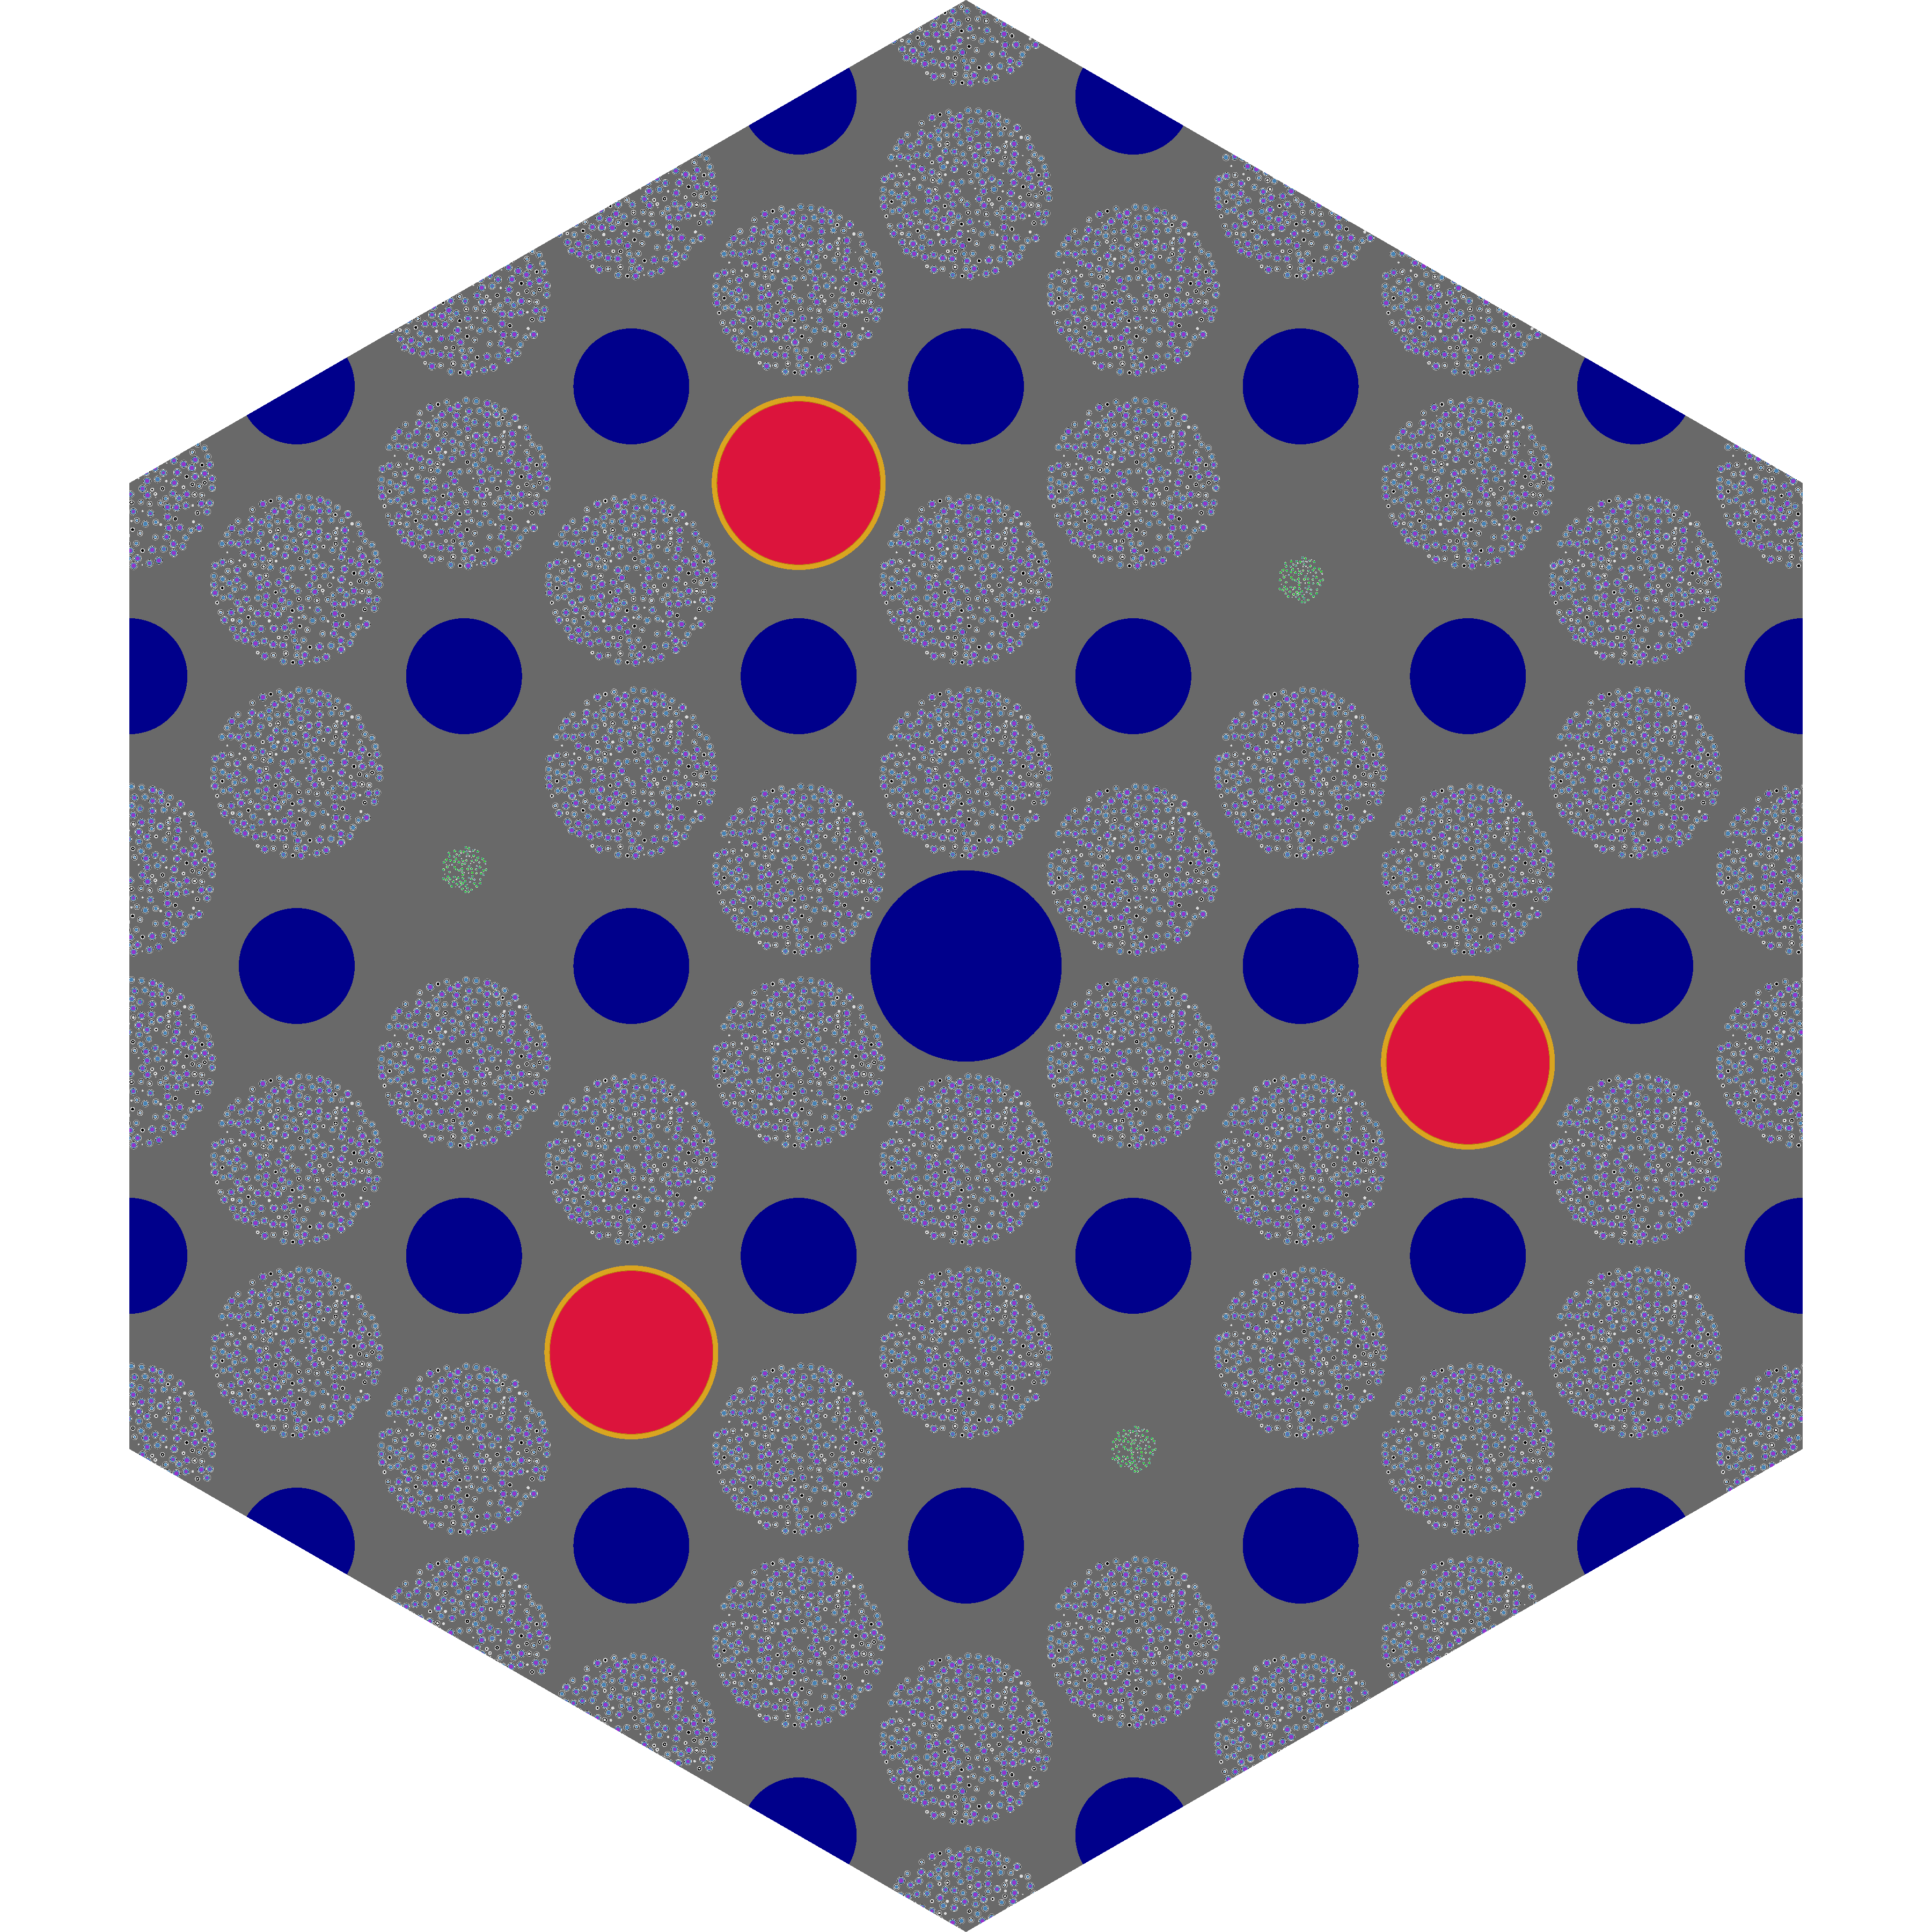
\includegraphics[width=0.9\linewidth]{figures/gcmr_slice.png}
            \end{figure}
        \end{minipage}
    \end{frame}
\end{withoutheadline}

\appendix

\begin{withoutheadline}
    \begin{frame}{System Parameters}
        \begin{table}[h]
            \centering
            \begin{tabular}{|c|c|c|}
                \hline
                \multicolumn{3}{|c|}{\textbf{geometric parameters}} \\
                \hline
                fuel compact radius & poison compact radius & moderator compact radius  \\
                \hline
                0.90 cm & 0.25 cm   & 0.843 cm  \\
                \hline
                control compact radius & coolant compact radius & FeCrAl thickness \\
                \hline
                0.99 cm    & 0.60 cm & 0.05 cm \\
                \hline
                Cr coating thickness & reflector heights & core height \\
                \hline
                0.007 cm & 20 cm & 160 cm \\
                \hline
            \multicolumn{3}{c}{} \\
            \multicolumn{3}{c}{} \\
            \hline
            \multicolumn{3}{|c|}{\textbf{operation and design parameters}} \\
            \hline
            fuel packing fraction & poison packing fraction  & enrichment \\
            \hline
            40\%  & 25\% &  19.95\% \\
            \hline
            inlet temperature & outlet temperature & outlet pressure \\
            \hline
            873.15 K & 1133.65 K  & 7 MPa \\
            \hline
            \end{tabular}
            \label{tab:operational_params}
        \end{table}
    \end{frame}
    \end{withoutheadline}

\begin{withoutheadline}
\begin{frame}{$\Delta \rho$ with $2\sigma$ error as a function of burnup  up to $\sim$29 GWd/tonne-U}
    \begin{figure}
        \hspace*{-1.35cm}
        \begin{subfigure}{0.5\linewidth}
            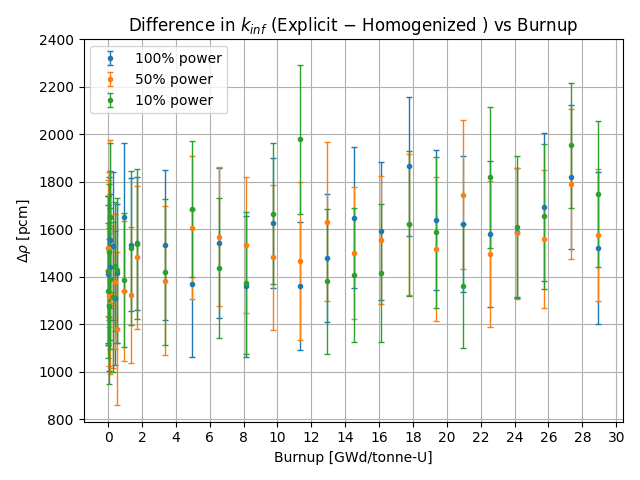
\includegraphics[width=1.175\linewidth]{figures/explicit_minus_homog.png}
        \end{subfigure}
        \begin{subfigure}{0.5\linewidth}
            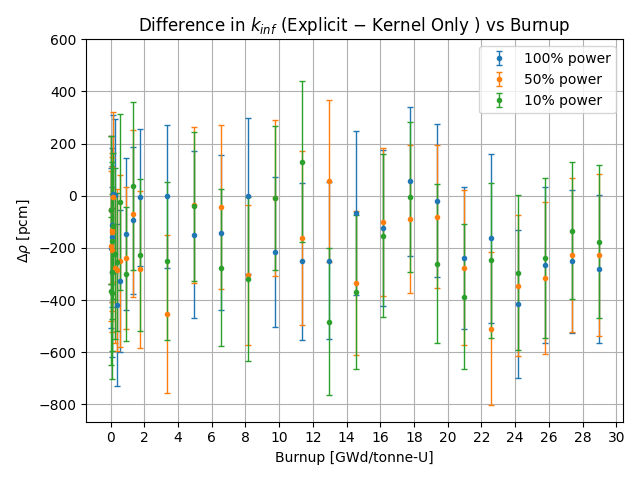
\includegraphics[width=1.175\linewidth]{figures/explicit_minus_kern.png}
        \end{subfigure}
        \label{fig:pcm_diffs}
    \end{figure}
\end{frame}
\end{withoutheadline}

\begin{withoutheadline}
\begin{frame}{Equilibrium Xenon-135 Number Densities}
    \LARGE
    \begin{table}
        \centering
        \caption{All units are atom per cubic centimeter. Since the first five time steps are used to converge xenon, the numbers below are the average of the fifth to the last value for xenon number density.}
        \begin{tabular}{|c|c|c|c|} \hline
        representation & explicit & kernel only & homogenized \\ \hline
        100\% power & $2.43127\times 10^{16}$ & $2.41845\times 10^{16}$ & $1.19125\times 10^{15}$ \\  \hline
        50\% power & $1.31047\times 10^{16}$ & $1.30864\times 10^{16}$ & $6.45668\times 10^{14}$ \\ \hline
        10\% power & $2.82398\times 10^{15}$ & $2.81919\times 10^{15}$ & $1.38810\times 10^{14}$ \\ \hline
        \end{tabular}
        \label{tab:xenons}
    \end{table}
    \begin{itemize}
        \item These equilibrium values explain the observed trend at fresh fuel -- and for much of the simulation -- that lower power with the same total burnup has more excess reactivity.
        \item The higher the power, the more Xenon-135 is produced during the initial jump to steady state, contributing to a larger negative reactivity insertion.
    \end{itemize}
\end{frame}
\end{withoutheadline}

\begin{withoutheadline}
\begin{frame}{Plutonium 241 at Each Power for the Fully Explicit Case}
    \begin{figure}
        \vspace*{-0.4cm}
        \centering
            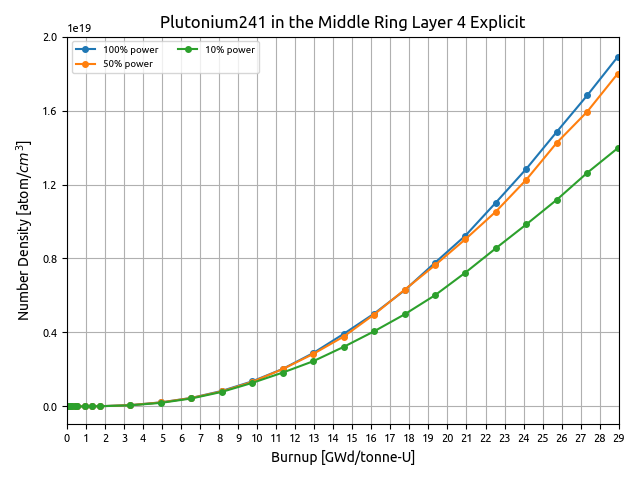
\includegraphics[height=0.9\textheight]{figures/explicit_Pu_241.png}
    \end{figure}
\end{frame}
\end{withoutheadline}

\end{document}
